\section{问题一:风化影响分析与成分恢复模型}

古代玻璃文物在长期埋藏过程中会发生风化作用,导致其表面化学成分发生改变。为探究风化作用对不同类别玻璃文物的影响,并尝试恢复其风化前的成分含量,本章建立了分析与预测模型。我们首先检验了表面风化与文物其他物理属性之间的统计关联,然后分析了风化对高钾和铅钡两类玻璃化学成分含量的影响规律,最后构建了一个基于风化系数的预测模型,用于推断风化样品的原始化学成分,其框架如图\ref{fig:问题一模型框架}所示。

\begin{figure}[H]
	\centering
	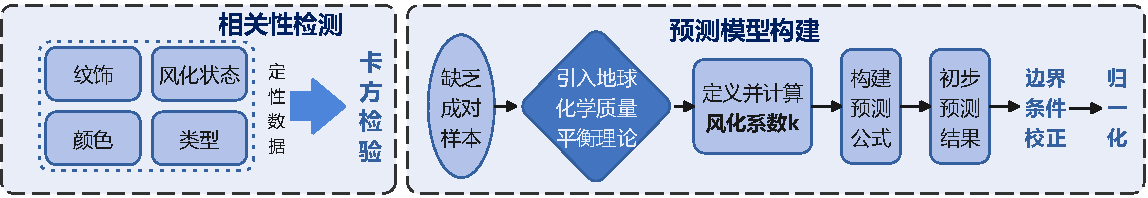
\includegraphics[width=\textwidth]{figs/3问题一/第一问框架.pdf}
	\caption{风化影响分析与成分恢复模型框架}
	\label{fig:问题一模型框架}
\end{figure}

\subsection{表面风化与文物物理属性的关联性检验}

为了探究文物表面风化现象是否与其物理属性存在关联,我们首先需要分析表面风化状态与玻璃类型、纹饰及颜色这几个变量之间的关系。这些变量的共同特征是它们均为分类变量,其取值为离散的类别而非连续的数值。

这一数据特性决定了用于衡量连续变量间线性关系的皮尔逊相关系数或用于比较组间均值差异的方差分析等方法在此并不适用,因为对“浅蓝”、“纹饰A”等类别进行数值运算不具备实际意义,需要采用一种能够处理定性数据频数的非参数检验方法来分析它们之间的关联性。因此,针对此问题,我们使用了卡方检验 ($\chi^{2}$ test)。

卡方检验 ($\chi^{2}$ test) 是一种专门用于判断两个或多个分类变量之间是否存在关联的经典统计方法,其核心思想在于比较观测频数与期望频数之间的差异。其中,观测频数是样本数据中各类组合的实际计数值,而期望频数则是在“变量间相互独立”这一零假设下,根据边际概率计算出的理论计数值。检验过程通过计算两者差异的卡方统计量,并将其转换为$P$值来进行判断。在本研究中,我们设定显著性水平为$0.05$,若计算所得的$P$值小于该阈值,则拒绝变量间相互独立的零假设,认为它们之间存在显著的统计学关联。

为直观分析文物表面风化现象与其物理属性的关联,我们制作了关系分析的可视化图,如图\ref{fig:关系分析可视化}所示。图中第一部分展示了风化状态在两类玻璃中的分布情况。数据显示,铅钡玻璃的风化样本占其总数的73.5\%,这一比例远高于高钾玻璃的33.3\%。图中第二部分与第三部分则进一步展示了风化样本在不同纹饰和颜色类别下的数量分布。所有纹饰为B的样本均为风化样本,而纹饰为A的样本中风化与未风化数量相同。在不同颜色中,浅蓝色样本的风化数量为20,远超其未风化数量6,而蓝绿色样本中两者的数量则基本持平。这些在不同类别下风化比例与数量的显著差异直观地表明表面风化与文物的物理属性并非相互独立。





\begin{figure}[H]

\centering

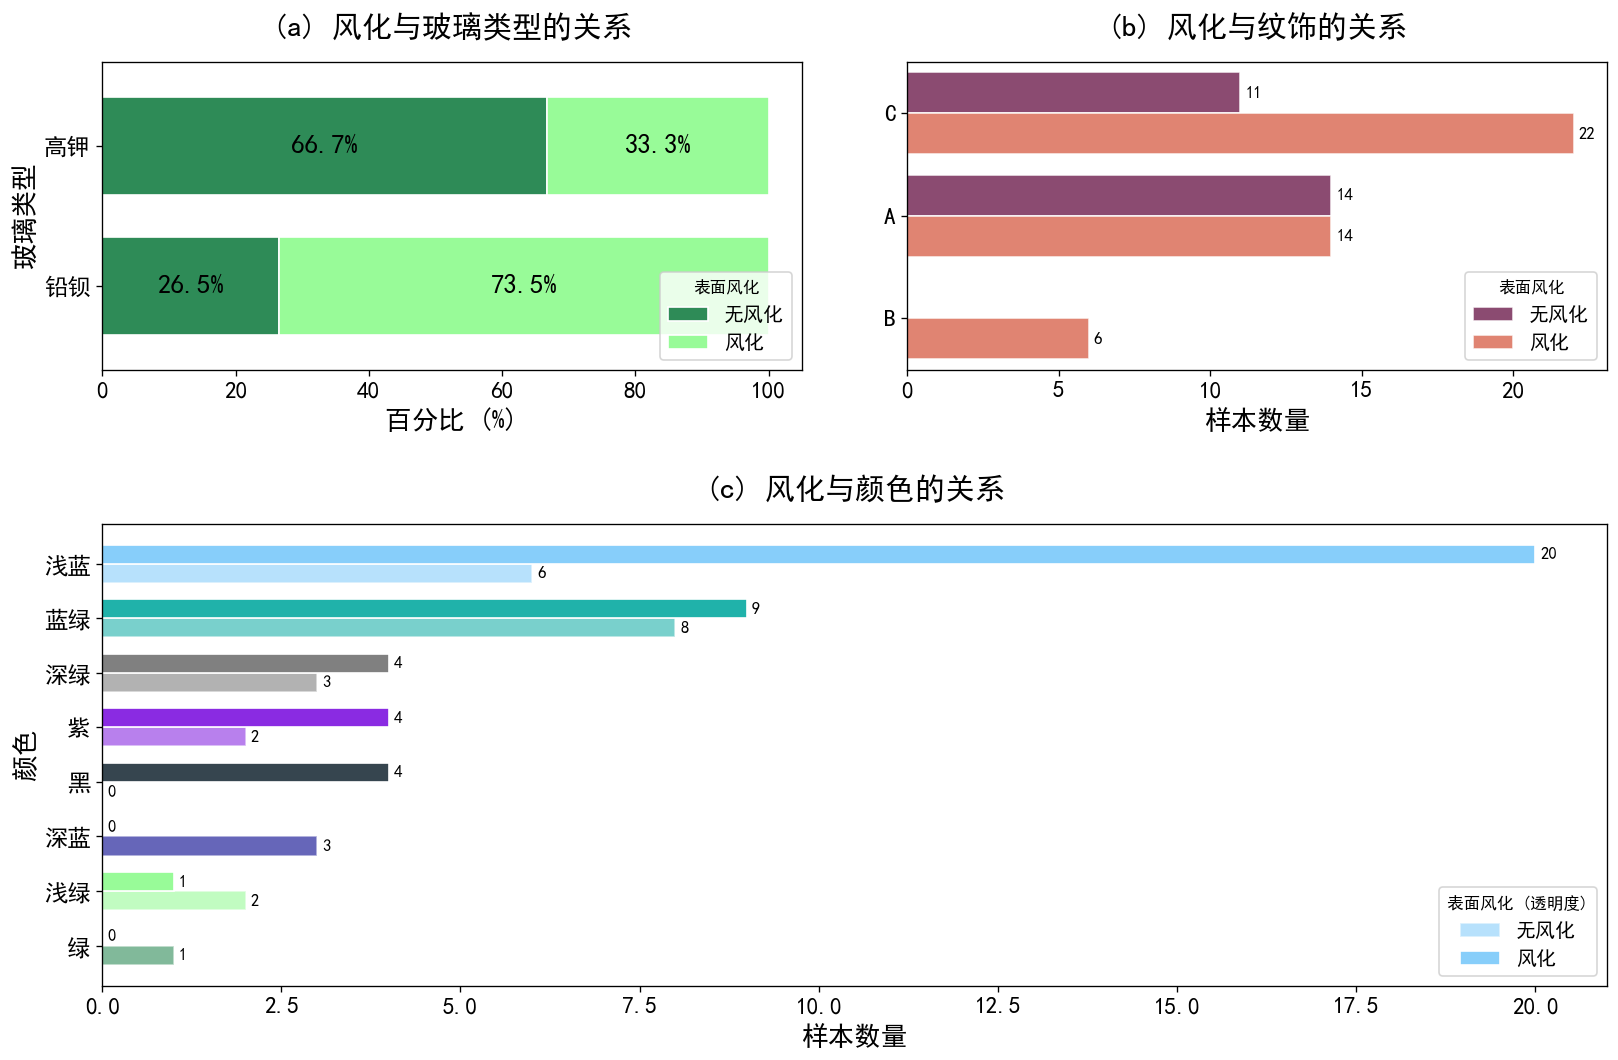
\includegraphics[width=\textwidth]{figs/3问题一/问题一_关系分析可视化_组合图_黄金分割.png}

\caption{表面风化与类型、纹饰及颜色的关系可视化}

\label{fig:关系分析可视化}

\end{figure}




\subsection{风化对两类玻璃化学成分含量的影响规律}

基于风化与玻璃类型存在关联的结论,我们进一步对风化在高钾和铅钡两类玻璃中引起的化学成分变化规律进行分析。我们将样本数据分为高钾未风化、高钾风化、铅钡未风化、铅钡风化四个组别,并对各组样本的化学成分含量分布进行了比较。

我们采用分面箱线图对两类玻璃在风化前后的化学成分分布进行可视化,如图\ref{fig:高钾玻璃成分分布}与图\ref{fig:铅钡玻璃成分分布}所示。箱线图展示了数据的中位数、四分位距和离散程度。从图中可以观察到,对于高钾玻璃,风化作用导致氧化钾$K_2O$的含量中位数显著下降,而氧化硅$SiO_2$的含量则有上升趋势。对于铅钡玻璃,风化作用主要表现为氧化铅$PbO$与氧化钡$BaO$含量的大幅降低,同时氧化硅$SiO_2$含量相应增加。这种变化说明风化过程中发生了元素的选择性流失与富集。

\begin{figure}[H]
	\centering
	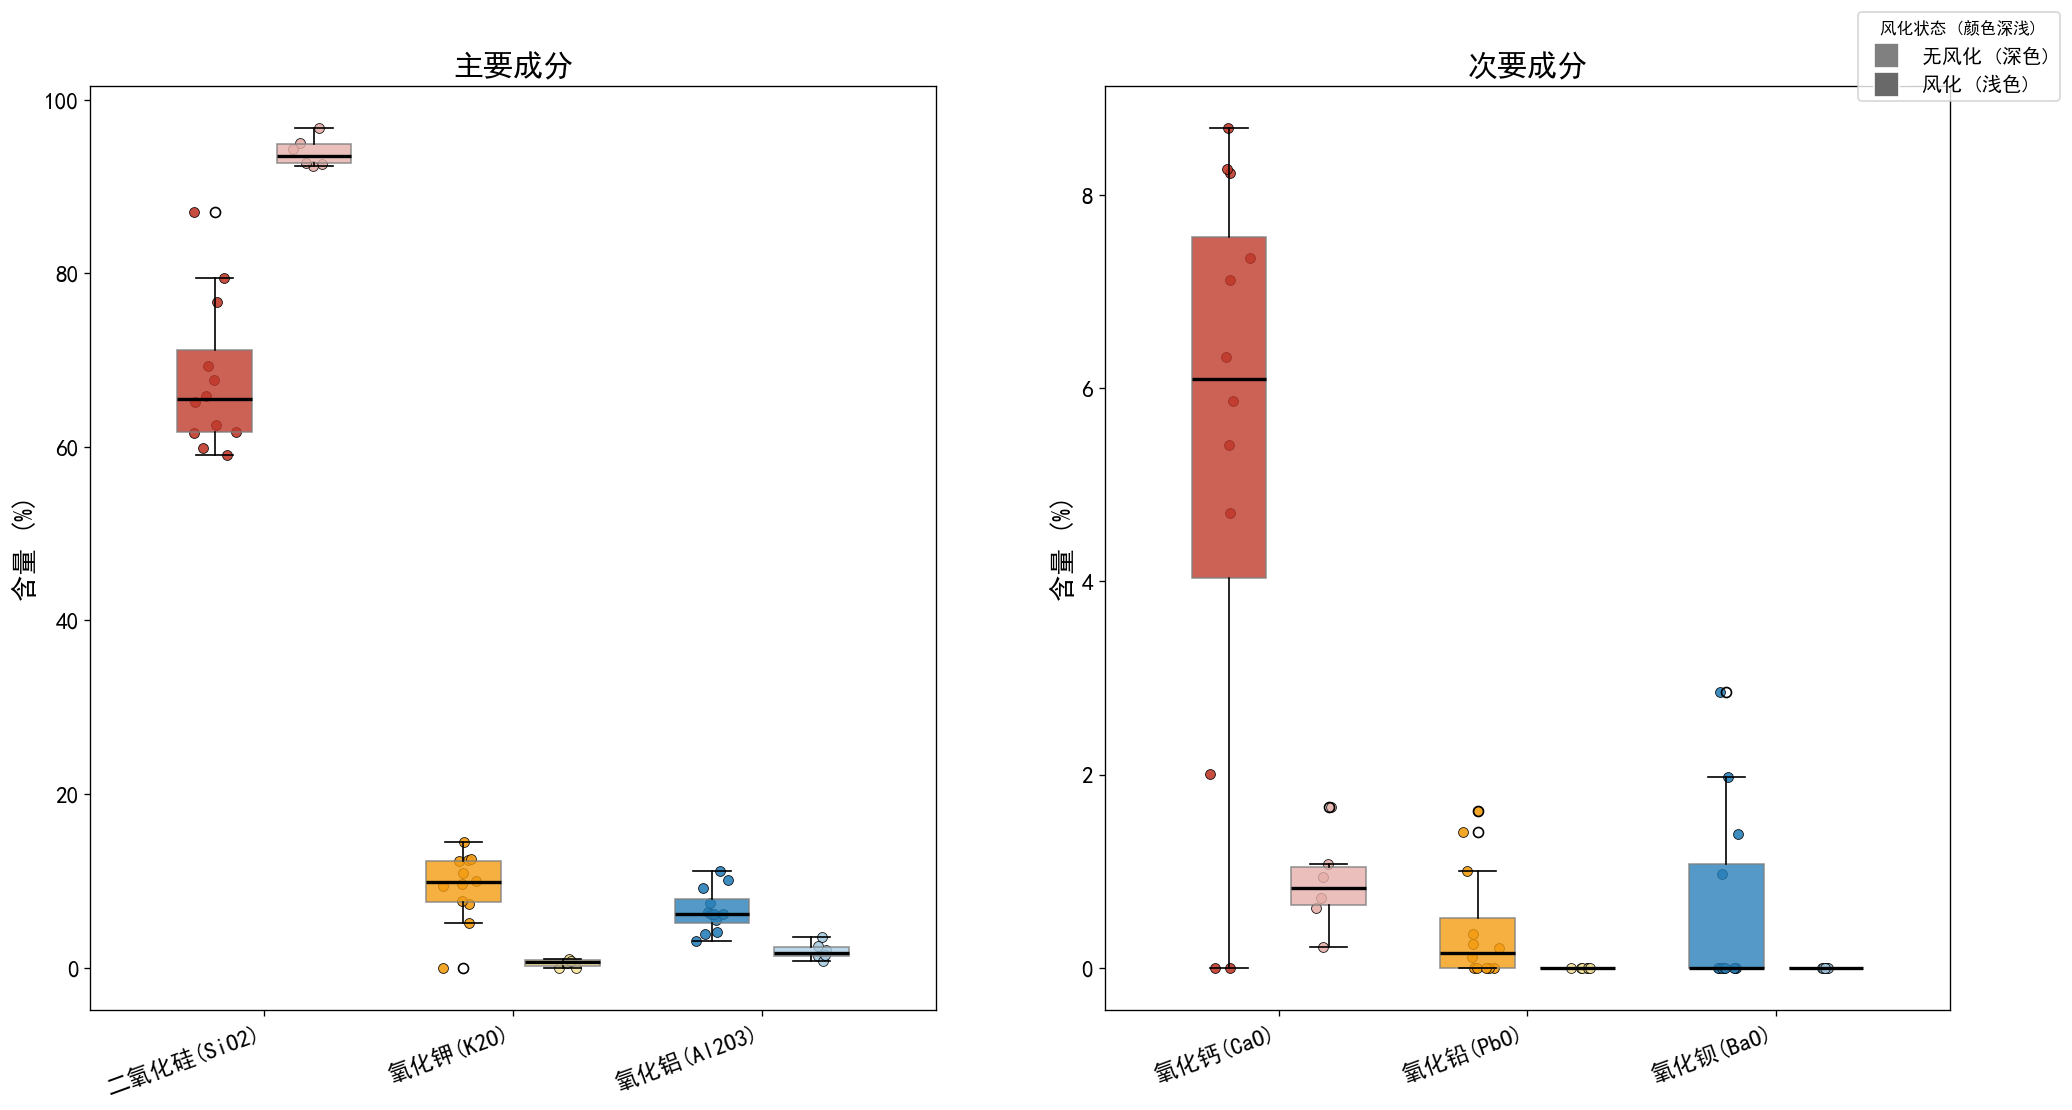
\includegraphics[width=\textwidth]{figs/3问题一/高钾玻璃成分分布.png}
	\caption{高钾玻璃在风化前后各化学成分含量分布}
	\label{fig:高钾玻璃成分分布}
\end{figure}

\begin{figure}[H]
	\centering
	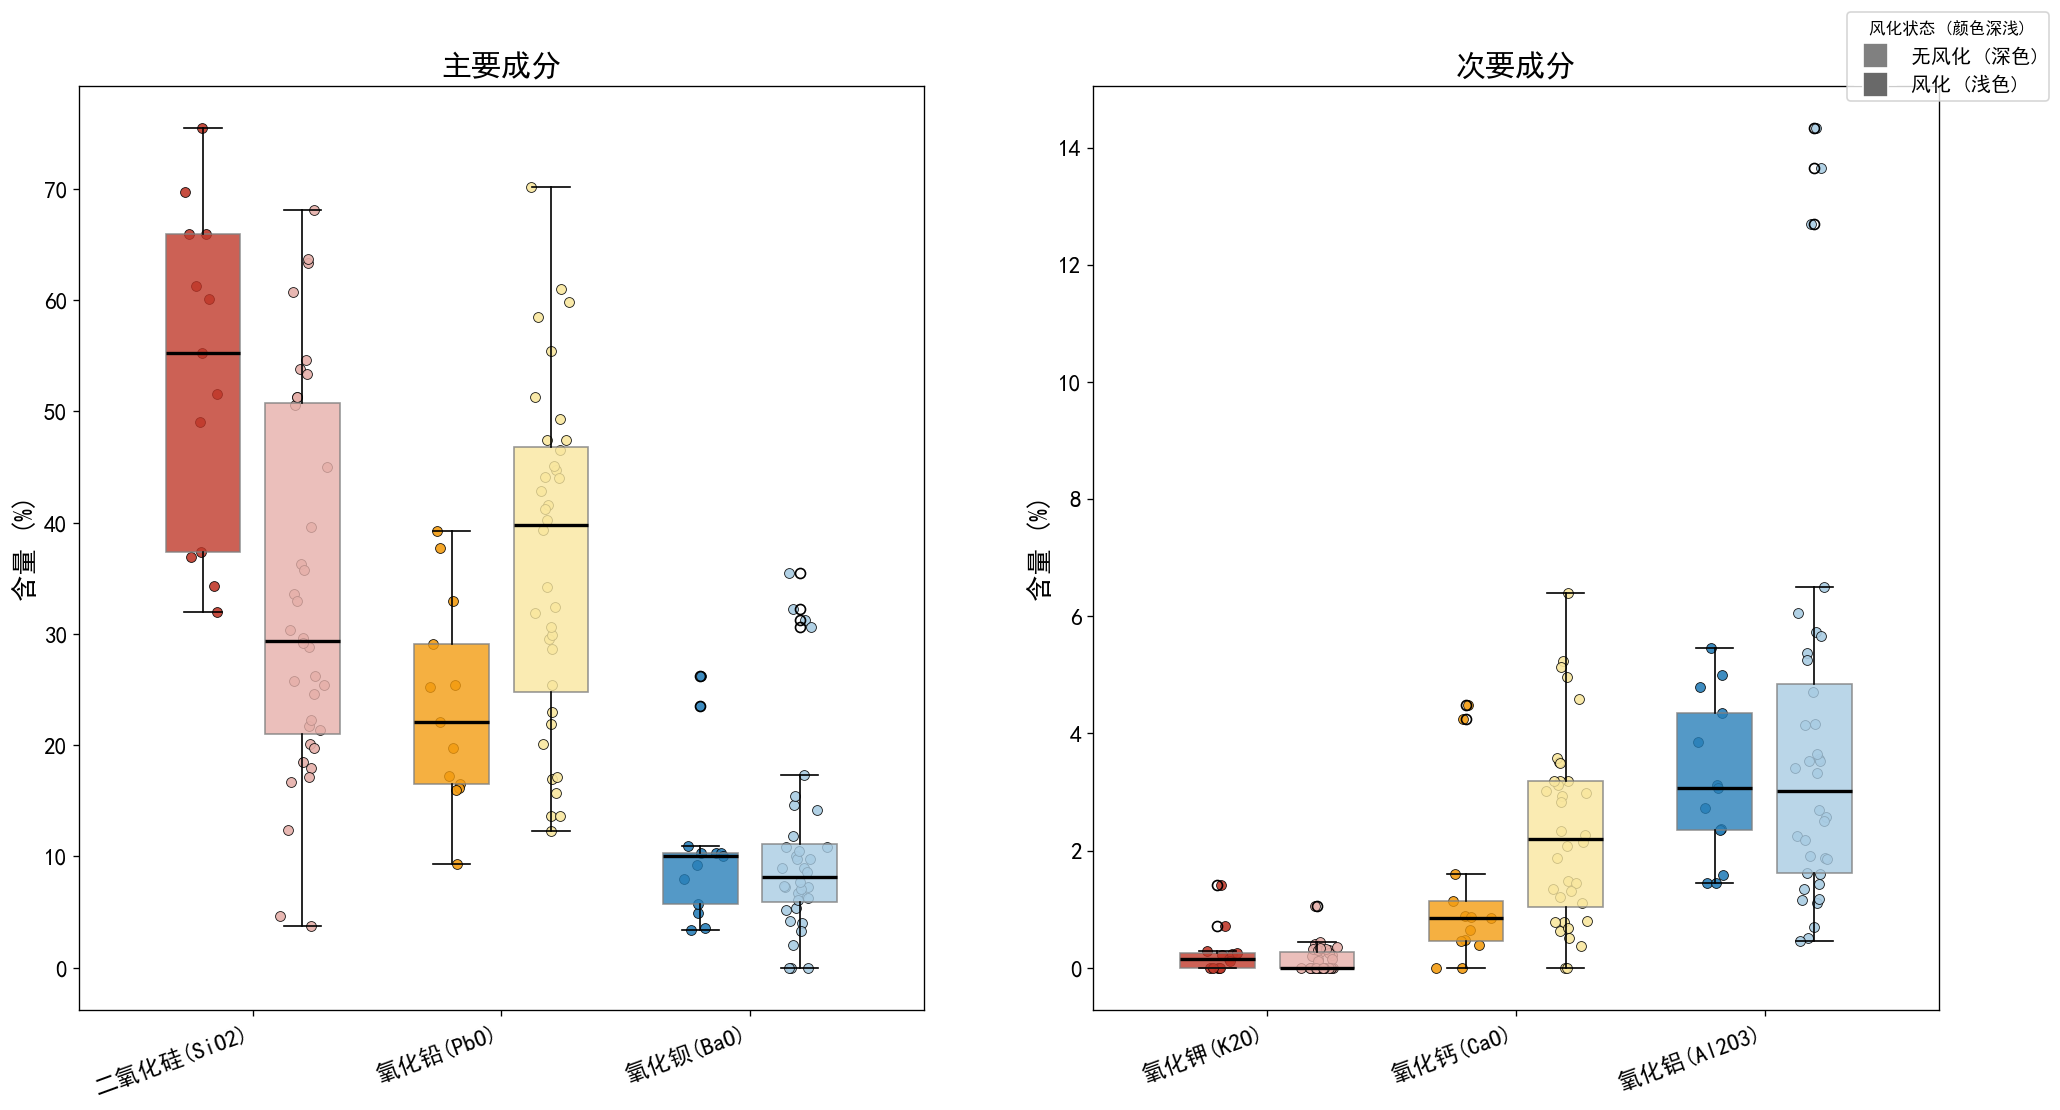
\includegraphics[width=\textwidth]{figs/3问题一/铅钡玻璃成分分布.png}
	\caption{铅钡玻璃在风化前后各化学成分含量分布}
	\label{fig:铅钡玻璃成分分布}
\end{figure}


为了更细致地观察关键化学成分的分布形态变化,我们绘制了部分核心化学成分,包括氧化铅$PbO$、氧化钾$K_2O$、氧化钡$BaO$以及二氧化硅$SiO_2$的分布图,如图\ref{fig:pbo_dist}至图\ref{fig:sio2_dist}所示。图中包含直方图与核密度估计曲线,它们共同描述了数据分布的集中趋势和形态。分析这些分布图可以发现,高钾玻璃在风化后,其氧化钾$K_2O$的含量分布从一个较宽的区间转化至接近零值的极低水平。对于铅钡玻璃,风化作用使其特征成分氧化铅$PbO$与氧化钡$BaO$的含量分布整体向低值区移动。与此相反,作为玻璃基体的二氧化硅$SiO_2$,其含量分布在两类玻璃中均表现出向高值区偏移的趋势,说明在风化过程中其他元素的流失导致了二氧化硅的相对富集。


\begin{figure}[H]
	\centering
	\begin{minipage}{0.48\textwidth}
		\centering
		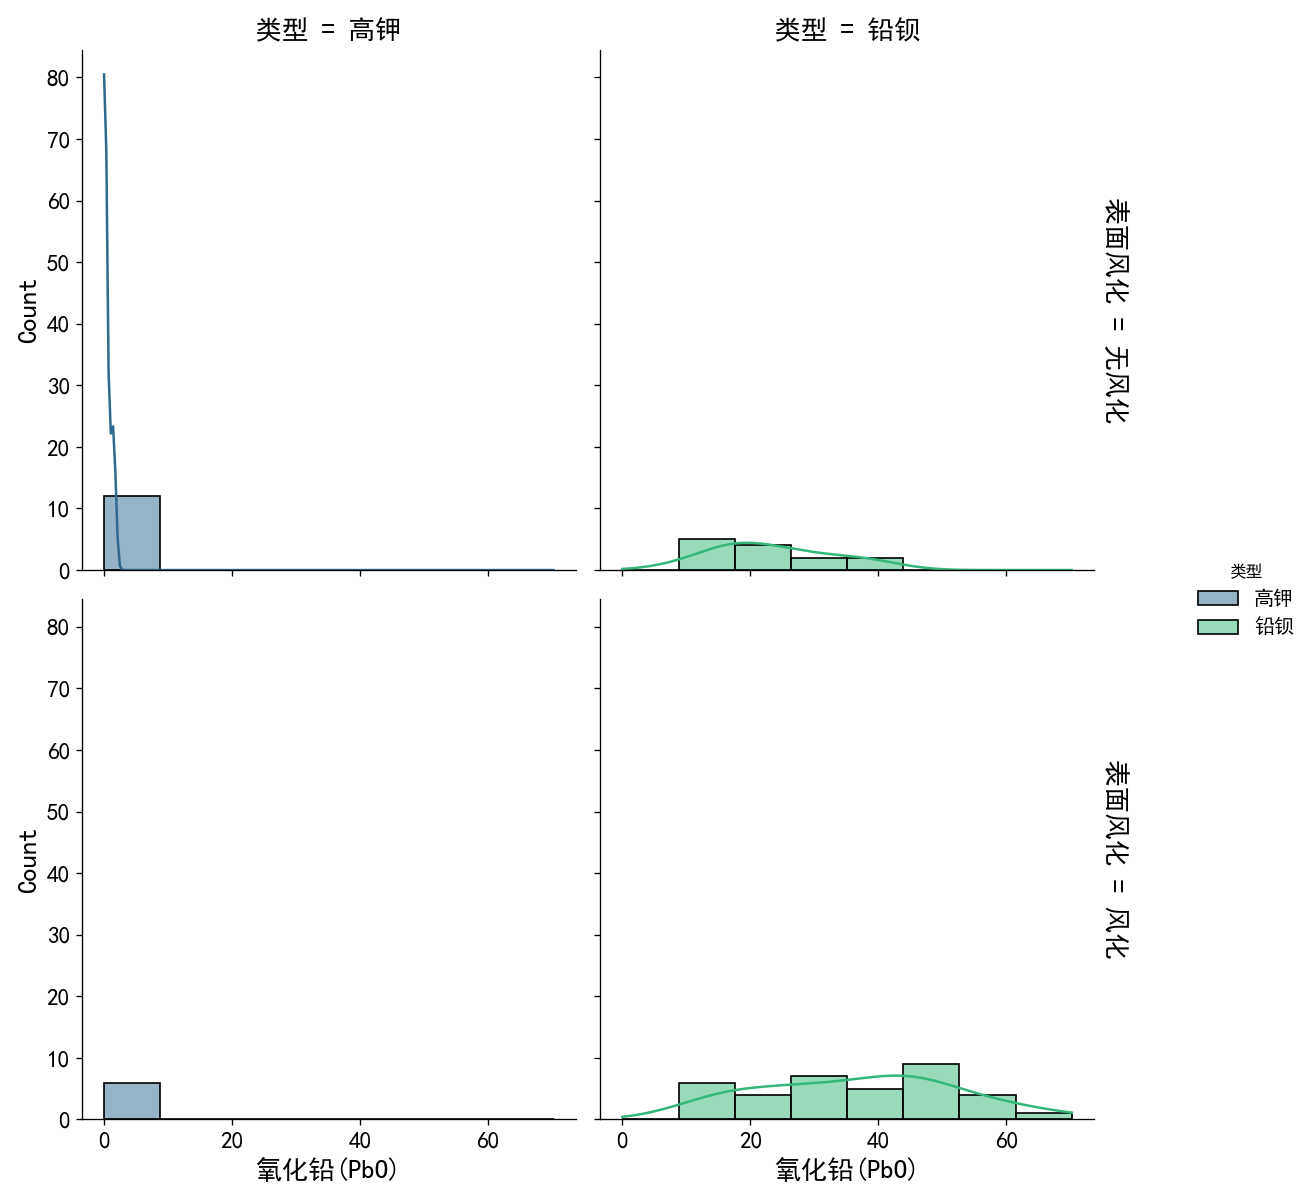
\includegraphics[width=\linewidth]{figs/3问题一/分布图_氧化铅(PbO).png}
		\caption{氧化铅$PbO$含量分布}
		\label{fig:pbo_dist}
	\end{minipage}\hfill
	\begin{minipage}{0.48\textwidth}
		\centering
		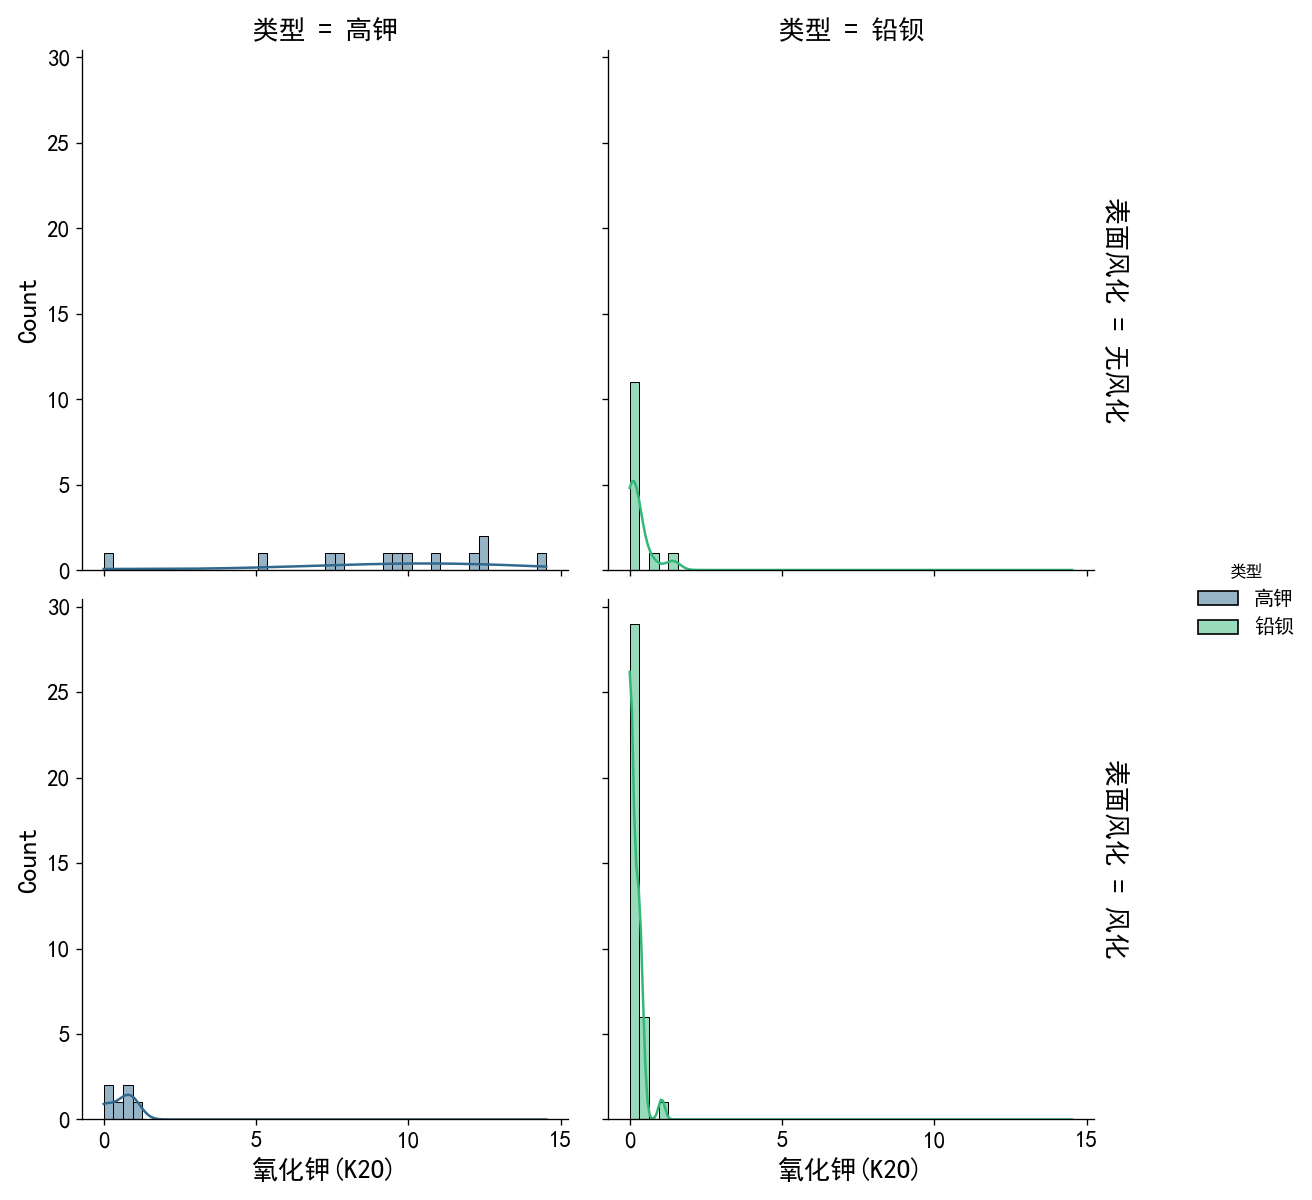
\includegraphics[width=\linewidth]{figs/3问题一/分布图_氧化钾(K2O).png}
		\caption{氧化钾$K_2O$含量分布}
		\label{fig:k2o_dist}
	\end{minipage}
\end{figure}

\begin{figure}[H]
	\centering
	\begin{minipage}{0.48\textwidth}
		\centering
		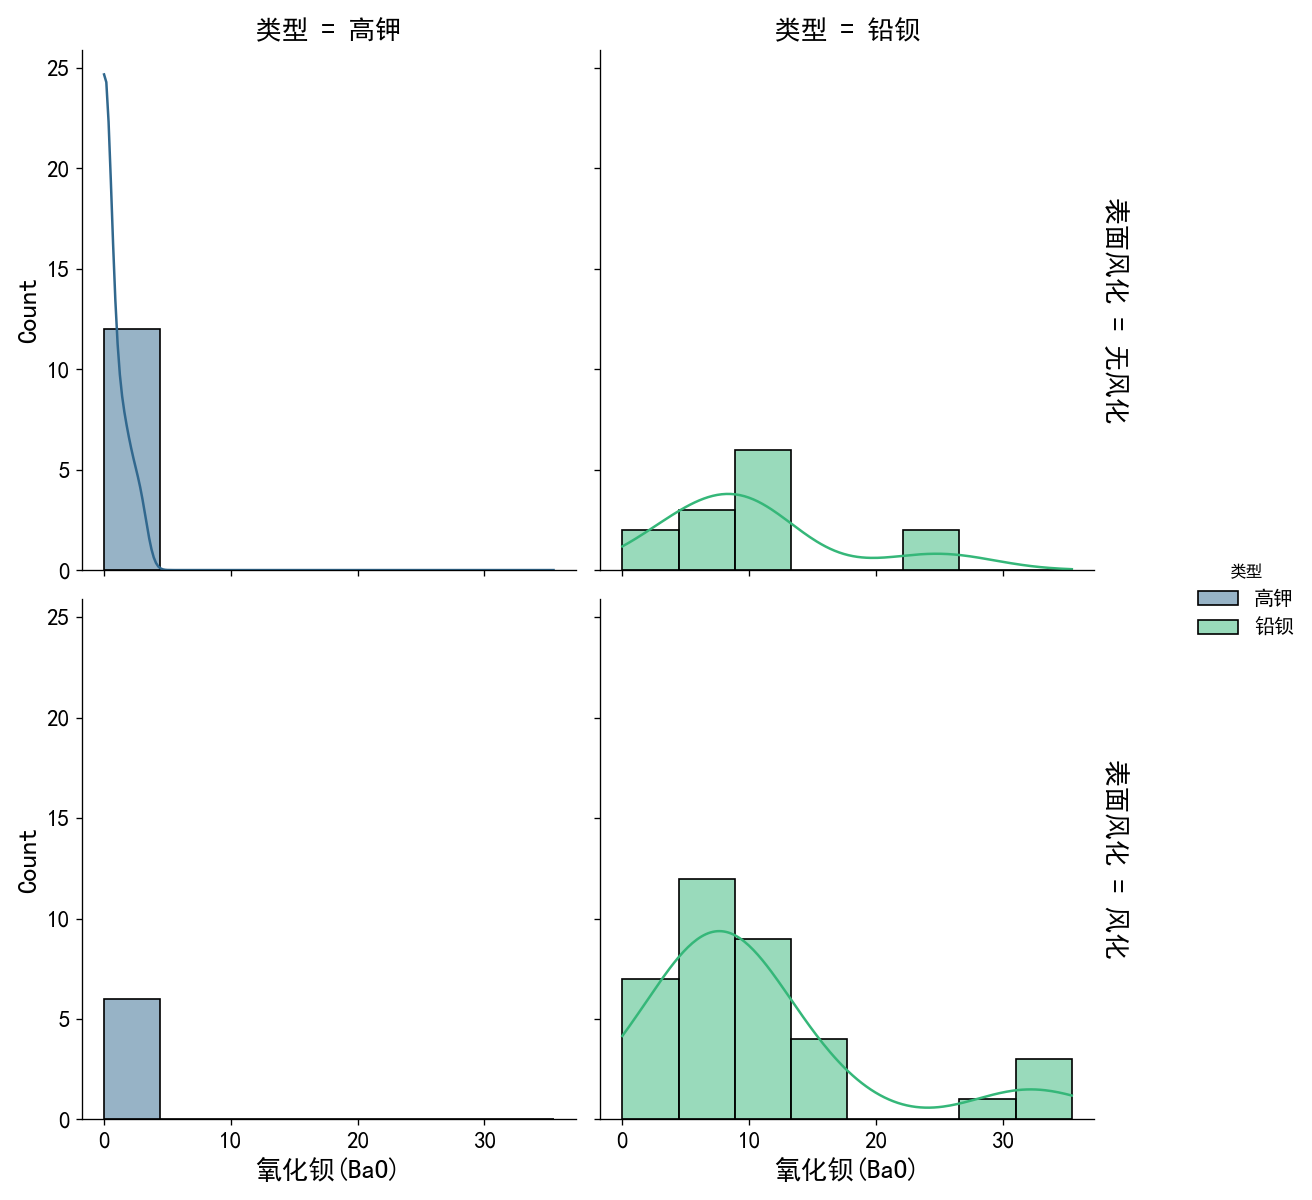
\includegraphics[width=\linewidth]{figs/3问题一/分布图_氧化钡(BaO).png}
		\caption{氧化钡$BaO$含量分布}
		\label{fig:bao_dist}
	\end{minipage}\hfill
	\begin{minipage}{0.48\textwidth}
		\centering
		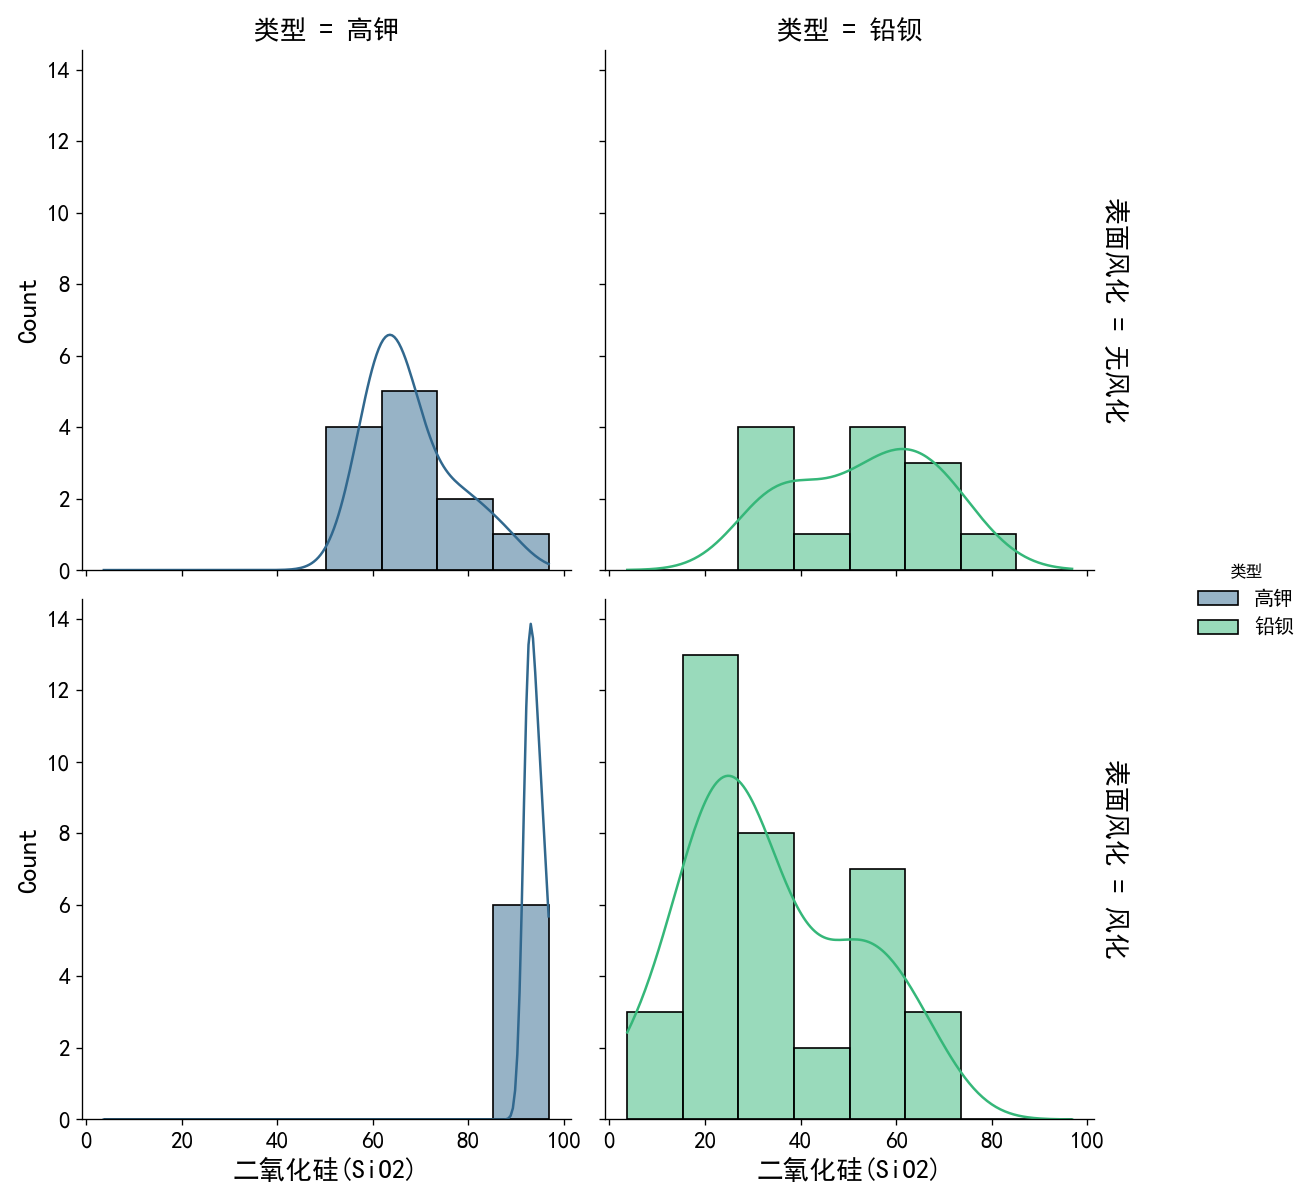
\includegraphics[width=\linewidth]{figs/3问题一/分布图_二氧化硅(SiO2).png}
		\caption{二氧化硅$SiO_2$含量分布}
		\label{fig:sio2_dist}
	\end{minipage}
\end{figure}

\subsection{基于风化系数的化学成分含量预测模型}

预测风化前化学成分的主要困难在于数据中缺乏源自同一文物的风化与未风化的观测样本。这使得依赖大量成对样本进行训练的传统监督学习模型,例如回归分析,难以直接应用且存在较高的过拟合风险。

于是,我们转向从风化过程的物理化学机理中寻求建模依据。玻璃的风化过程与地质学中岩石的蚀变过程在原理上具有相似性,均为长期化学环境作用下的元素迁移过程。因此,我们引入了地球化学领域成熟的质量平衡分析理论来构建预测模型,该理论能够在缺乏直接演变过程数据时,对成分变化进行有效推断。

我们的模型的核心假设为:特定化学成分在风化过程中的流失或富集比例,与其在未风化状态下的原始含量相关。此假设参考了地质学中分析交代蚀变作用的艾索康图法的原理,它将风化视为一个系统性的化学变化过程而非随机过程,从而建立了基于风化系数的预测方法。

我们首先为每种玻璃类型$t$和每种化学成分$j$定义一个风化系数$k_{t,j}$。该系数由该类型玻璃中所有风化样本与未风化样本的平均含量计算得出,其数学表达式如下:
\begin{equation}
	k_{t,j} = 1 - \frac{\bar{C}_{t,j,\text{weathered}}}{\bar{C}_{t,j,\text{unweathered}}}
\end{equation}
其中,$\bar{C}_{t,j,\text{weathered}}$表示$t$类玻璃风化样本中$j$成分的平均含量,$\bar{C}_{t,j,\text{unweathered}}$表示$t$类玻璃未风化样本中$j$成分的平均含量。

利用计算得到的风化系数,我们可以对任意一个已知风化后成分含量$C_{\text{weathered}, j}$的样本,进行其风化前含量$C'_{\text{unweathered}, j}$的初步预测,其预测公式为:
\begin{equation}
	C'_{\text{unweathered}, j} = \frac{C_{\text{weathered}, j}}{1 - k_{t,j}}
\end{equation}

考虑到测量误差和模型的局限性,初步预测得到的各成分总和可能偏离100\%。因此,我们对预测结果进行了边界条件校正。我们计算所有预测成分的总和,并进行条件归一化处理,以确保最终得到的预测成分总和落入题目要求的85\%至105\%的有效区间内,从而使预测结果在化学上更具合理性。模型的最终预测结果,以原始含量和预测含量并列对比的形式,被完整地保存至\texttt{Result/问题一\_预测结果.xlsx}文件中。

